\graphicspath{{../01Introduction/pics/}}

\chapter{Introduction}\label{ch:Introduction}

\begin{quoting}
	This quantum business is so incredibly important and difficult that everyone should busy himself with it. 
	
	
	A. Einstein in a letter to his friend Jakob Laub in 1908, as quoted by A. Wheeler in “The Mystery and The Message Of The Quantum”
\end{quoting}

{\bf Abstract}\hspace{0.2cm} In this chapter.


\lettrine[lines=2]{\color{darkocre}Q}{uantum physics is a century-old branch of physics. Its success} is unparalleled and yet quantum physics is unfinished in one sense: There is no clear and widely adopted consensus on what some of quantum ideas "really mean."

\section{What Is Quantum Physics?}
There are many characterizations of quantum physics.  In essence, quantum physics is the part of physics which focuses on \emph{quantum systems} -- physical systems showing \emph{quantum behavior}. So, what effects or phenomena are quantum?


\section{Brief Historical Context}
The year 1900 is usually considered the birth year of quantum physics. On December 14 of 1900, at the meeting ????, the German physicist Max Karl Ernst Ludwig Planck presented his theoretical explanation of the \emph{spectrum} of electromagnetic radiation emitted by hot bodies. In his work he introduced what is now known as \emph{Planck's constant}  $h$, which has a physical meaning of \emph{elementary quantum of action}.
\begin{mybio}{Niels Bohr On $h$}
	The Danish physicist Niels Bohr, one of the founders of quantum physics, wrote: 
	
	\emph{
	"A new epoch in physical science was inaugurated, however, by Planck’s discovery of the elementary quantum of action, which revealed a feature of wholeness inherent in atomic processes, going far beyond the ancient idea of the limited divisibility of matter."
}
	
	(Atomics Physics and Human Knowledge, Quantum Physics and Philosopy, Complimentarity and Causality.)
\end{mybio}
Let's take a look at what happened before and after Planck's discovery.

\subsubsection*{Pre-History: Spectroscopy and Molecular Theory}
The evolution of physics in the century preceding quantum era is fascinating. It is important to know some of pre-history in order to appreciate the context in which quantum physics was born. We will highlight two big advancements, one in experimental, and the other in theoretical departments. 

\subsubsection*{Spectroscopy}
First, the methods of \emph{spectroscopy}--study of energy distribution across various wavelengths of visible and invisible light--experienced significant development. Already in 1802 an English chemist and physicist William Hyde Wollaston observed that\footnote{Wollaston William Hyde 1802 XII. \emph{A method of examining refractive and dispersive powers, by prismatic reflection}, Phil. Trans. R. Soc. {\bf 92}: 365–380 } "If a beam of day-light be admitted into a dark room by a crevice 1/20 of inch broad\footnote{1/20 in = 1.27 mm.}, and received by the eye at the distance of 10 or 12 feet\footnote{10-12 feet = 3-3.7 m.}, through a prism of flint glass" one can see four colors (red, yellowish green, blue, and violet) separated by \emph{dark lines}. Soon many more dark lines in the optical spectrum of the Sun were discovered and systematically studied by a German physicist Joseph Ritter von Fraunhofer. Today these \emph{Fraunhofer lines} are understood to result from the \emph{absorption} of radiation by different atoms in the atmospheres of the Sun and earth.
\begin{figure}[htbp]
	\centering
	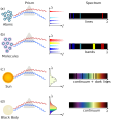
\includegraphics[scale=1.0]{spectraTypes}
	\caption{Various types of spectra observed from different substances. (a); (b); (c); (d). See text for explanation.}
	\label{fig:spectraTypes}
\end{figure}


The energy absorbed by a substance can be \emph{emitted}. The study of \emph{emission spectra} from various bodies revealed a great deal of complexity and provided a lot of information about bodies' material composition and state. 

There are four basic types of spectra one can observe, as illustrated in Figure \ref{fig:spectraTypes}. In a typical spectroscopic observation radiation from an excited object is sent through a \emph{dispersive} component, such as a prism or a diffraction grating\footnote{See Visual Glossary}. A beam of radiation is spread out according to colors and light of different color falls at different place of a detector (eye, photographic plate, or an electronic camera).

Light emitted by atoms consists of very definite colors which show up as \emph{emission lines} in spectra, as shown in Figure \ref{fig:spectraTypes}(a). Exact locations of such lines tell which atom emits the radiation. Simpler atoms, such as hydrogen or helium, have simpler spectra.

Spectra of excited molecules contain many closely placed lines. Sometimes multiple lines coalesce into a \emph{band}, as in Figure \ref{fig:spectraTypes}(b).

Radiation from large hot bodies, like Sun, reveals both discrete and continuous color distribution; see Figure \ref{fig:spectraTypes}(c). All colors are present in the spectrum, and dark Fraunhofer lines indicate that some of the radiation has been absorbed on its way to the detector by atoms and molecules.

Finally, an important radiation type corresponds to an \emph{idealized} object, called \emph{black body} -- a theoretical material which does not relfect any incident radiation. In other words, \emph{black body absorbs all incoming radiation}. Of course, black body also emits radiation, otherwise it would never stop accumulating energy from incident light. Therefore, black body \emph{is not truly black}, its perceived color depends on the temperature of the body. Emission spectrum of black-body, called \emph{black body radiation} or \emph{normal spectrum}, is of great interest, because it approximates emission spectrum from \emph{any material} kept at a constant temperature.
At the end of the 19th century, black body radiation was actively studied both experimentally and theoretically. 

\begin{mybio}{Max Planck And Black Body Radiation}
	Since black-body radiation spectrum does not depend on particular material, it has a universal nature. This fascinated Max Planck, as he wrote in his Scientific Autobiography\footnote{Max Planck, \emph{Scientific Autobiography and Other Papers}, Williams \& Norgate, 1950, pp. 34-35.}:
	
	\emph{"Thus, this so-called Normal Spectral Energy Distribution represents something absolute, and since I had always regarded the search for the absolute as the lofties goal of all scientific activity, I eagerly set to work."}
	
	\[
	\delta E = \rho\delta \nu = \frac{8\pi h\nu^3\delta\nu}{c^3}\frac{1}{e^{h\nu/kT}-1}\,.
	\]
\end{mybio}

The spectrum of black body radiation was the first type of spectrum to receive a theoretical explanation and an explicit formula. Spectra of atoms and molecules were properly studied only after the development of quantum mechanics.

Spectroscopy of the 19th century\footnote{William McGucken, \emph{Nineteenth-Century Spectroscopy}, The Johns Hopkins Press, 1969.}

\subsubsection*{Molecular Theory}
Second advancement of pre-quantum physics was connected with the hypothesis of atoms and molecules. Although atomistic ideas had been known for about two millenia, even in the 19th century far from every physicist was convinced that atoms and molecules were objects just as real as everyday things. There was no \emph{direct evidence} for the existence of atoms and molecules, and the main support for the atomistic views came from \emph{indirect evidence}, like the many useful results that followed from molecular theory. For example, the behavior of gases (diffusion, viscosity, laws connecting pressure and temperature, heat capacity, etc.) was especially well explained. Two major figures in this field were the Scottish physicis James Clerk Maxwell and the German physicist Ludwig Boltzmann.

In September of 1899, at the congress of the German Society of Natural Scientists and Physicians,  Ludwig Boltzmann presented a review titled \emph{"The Recent Development of Method In Theoretical Physics."}\footnote{\emph{The Monist}, January, 1901, Vol. {\bf 11}, No. 2, pp. 226-257.} He highlighted the rapid development of physics in the 19th century and discussed major experimental and theoretical results.

\begin{mybio}{Boltzmann's Prediction}
	\emph{"I have to mention finally the relations which obtain according to the molecular theory between the principle of entropy and the calculus of probabilies, concerning the real significance of which there may be some difference of opinion, but which, no unprejudiced person will deny, are eminently qualify to extend our intellectual horizon and to suggest new combinations both of ideas and experiments."}
\end{mybio}
Boltzmann's anticipation that "the principle of entropy and the calculus of probabilities" will lead to "new combinations both of ideas and experiments" was fully confirmed by Max Planck in about a year!

As explained in the Section XX, Max Planck used nearly the same approach as Boltzmann to calculate entropy of a thermodynamic system. Only in his case, the system was not an ideal gas of molecules, but a collection of oscillating molecules that interact with electromagnetic radiation (in the form of heat).


\subsection{Three Ages of Quantum}
The evolution of quantum science and technology can be roughly divided into three stages: (a) "Old quantum physics" (b) modern quantum physics, and (c) information-age quantum physics (see Figure \ref{fig:quantumTechnologyEvolution}).
\begin{figure}[htbp]
	\centering
	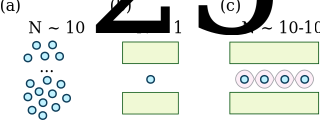
\includegraphics[scale=1.0]{quantumTechnologyEvolution}
	\caption{Three stages of quantum science and technology: (a) Observation of large groups of objects (atoms, molecules); (b) Study of interaction between single particles (one atom + one photon); (c) Connecting tens and hundreds of quantum systems using \emph{entanglement}.}
	\label{fig:quantumTechnologyEvolution}
\end{figure}



\subsubsection*{Old Quantum Physics}

\subsubsection*{Modern Quantum Physics}

\subsubsection*{Information Age}


\section{Who Needs Quantum Physics?}

In October of 1912, Albert Einstein\index{Einstein} wrote in a letter to his physicist
friend Arnold Sommerfeld:
\begin{mybio}{Example of mybio environment}
  I am now exclusively occupied with the problem of gravitation theory
and hope, with the help of a local mathematician friend, to overcome
all the difficulties. One thing is certain, however, that never in my
life have I been quite so tormented. A great respect for mathematics
has been instilled within me, the subtler aspects of which, in my stupidity,
I regarded until now as a pure luxury. Against this problem [of
  gravitation] the original problem of the theory of relativity is
child’s play.
\end{mybio}
In the period from 1905 to 1916 Einstein was feverishly working on the
General Theory of Relativity\index{General relativity} -- the next
best theory of gravity since
Newton. The mathematics of general relativity is based on the calculus
of tensors, created by Italian mathematicians Ricci-Curbastro and
Levi-Civita roughly a decade before Einstein started working on the
problem of gravity.


\section{Why is Quantum Physics Hard?}\label{sec:WhyQuantumHard}
Quantum physics is not an easy subject.  Mastering it requires learning new physical concepts and advanced mathematical tools. Additionally, it is necessary to examine critically some basic intuitive notions of classical physics and everyday experience.  All this takes time and effort.

\begin{mybio}{Feynman on Quantum Physics}
	In his book {\it The Meaning of It All}, Richard Feynman -- an American theoretical physicist and Nobel laureate -- wrote:
	
	
	"Trying to understand the way nature works involves a most terrible test of human
	reasoning ability. It involves subtle trickery, beautiful tightropes of logic on which one
	has to walk in order not to make a mistake in predicting what will happen. The quantum
	mechanical and the relativity ideas are examples of this."
	
	
	{\it The Meaning of It All, Section I: The Uncertainty of Science.}
\end{mybio}

Let us examine those features of quantum physics that make it particularly challenging and discuss what can be done to make the learning easier.

\subsection{Indirect Experience}
Concepts of classical physics, especially when applied to macroscopic objects, can often be connected to our experiences. Velocity, heat, force, pressure, motion of projectiles, currents of fluids, propagation of sound and so on -- all can be felt, seen, or otherwise perceived by humans. In contast, \emph{we do not have a direct access to the quantum side of the world.}  There are no experiments where one can say "Here, look at this entanglement!" or "Hey, touch this quantum of action!", or "Listen carefully, that is the decoherence!"

\begin{analogy}
	Imagine you want to understand the life of inhabitants of extremely distant land. The environment and climate of that land makes it impossible for you to travel there and see everything with your own eyes. 
	
	Who knows, maybe they do not have such notions as "home", "road", "tomorrow", "force", and so on.
	
	Now, if by "understand" we mean "explain and predict the behavior of aliens in our own terms", then the task might be hopeless. However, if by "understand" we mean "develop new concepts that describe and predict the behavior of aliens" then we might have a chance. Of course, the new concepts might be very foreign to us, at first. But the more we use them -- the less our mind struggles.
\end{analogy}


The problem then becomes two-fold. First, we need give up our non-quantum intution. Remember, our intution and conceptual pictures are rooted in macroscopic reality. We interact with the latter using our macroscopic organs and instruments which are unable to capture subtle non-classical features of the world. 

Second, we need to develop new intution and set of "pictures"/models which would be adequate for quantum world. While doing so, we must be careful not to "contaminate" this new way of thinking with old concepts. 

\subsection{Abstract Mathematics}
The mathematics used in modern physics is becoming increasingly more abstract. It is the price to pay for the powerful and general tools which are indespensible for expressing most advanced results of physics, either  classical or quantum.

Quantum physics does not use any special mathematical methods which would make it more challenging than classical physics. Of course, a student learning quantum theory might struggle with the heavy use of operators, complex vectors,  Hilbert spaces, commutators, matrices and so on. The difficulty, however, is not due to the quantum nature of the subject, since nearly all these mathematical concepts and tools could be found in other -- non-quantum -- areas of mathematical physics.

\begin{mybio}{Alfred Whitehead on Abstract Mathematics}
	Nothing is more impressive than the fact that as mathematics withdrew increasingly into the upper regions of ever greater extremes of abstract thought, it returned back to earth with a corresponding growth of importance for the analysis of concrete fact. ...The paradox is now fully established that the utmost abstractions are the true weapons with which to control our thought of concrete fact
	
	{\it Mathematics as an Element in the History of Thought, Ch. 2, p. 46}
\end{mybio}

Surprisingly, current mathematical framework of quantum physics is the simplest possible. Quantum theory is \emph{linear}, meaning that it is based on the \emph{superposition principle} and uses the \emph{simplest} kinds of operators -- \emph{linear operators}. It must be noted that the linearity is not exclusive to quantum theory, as, for example,  classical electrodynamics is also a linear theory.


\subsection{Inadequate Language}
Perhaps the biggest barrier on the path to mastering quantum physics is... \emph{ordinary language}. It has developed to communicate everyday experiences and emotions, but subtle natural phenomena are far removed from either of those.

\begin{mybio}{Bertrand Russell On Ordinary Language}
Ordinary language is totally unsuited for expressing what physics really asserts, since the words of everyday life are not sufficiently abstract. Only mathematics and mathematical logic can say as little as the physicist means to say.

{\it The Scientific Outlook (1931)}
\end{mybio}

\begin{mybio}{Werner Heisenberg On Ordinary Language}
	It is not surprising that our language should be incapable of describing the processes occurring within the atoms, for, as has been remarked, it was invented to describe the experiences of daily life, and these consist only of processes involving exceedingly large numbers of atoms. Furthermore, it is very difficult to modify our language so that it will be able to describe these atomic processes, for words can only describe things of which we can form mental pictures, and this ability, too, is a result of daily experience.
	
	{\it Principle of Quantum Theory (1930), Introductory, p. 11}
\end{mybio}
 
To capture deep and nuanced laws of nature, we must use a language of adequate power, built with new words and symbols completely foreign to common intuition and simple mental pictures. In other words, the adequate language has to be \emph{abstract}, \emph{purposefully developed}, and most likely \emph{unintuitive} to an untrained mind.
 
\begin{remark}
	Constructing new languages is a standard task in the field of computer science. New languages are regularly proposed to better describe computational tasks in a specific domain. For example, a separate language exists for working with database requests.
	
	In this field, a \emph{domain specific language} is usually developed to address problems 
	
	A language is considered good if it does not allow constructing meaningless or harmful statements. For example, if a language allows definition of a set of sets which are not elements of themselves, the this language will be plagued with the famous Russell paradox.  
	
	Natural human language is notoriously bad for formulating precise and abstract results of science.
\end{remark}

\begin{myrem}{Particles}
	Particles are excitations of quantum fields. They correspond to irreducible unitary representations of Lorentz group. Fields are operator-valued vector functions defined over Minkowski space and transformed simply under the action of the Poincare group.
\end{myrem}
Learning this language is the key to success. 

\section{Quantum Versus Classical}
When do we have to use quantum physics? Where is the border between quantum and classical phenomena?

\begin{figure}[htbp]
  \centering
  
\includegraphics[scale=1.0]{defaultFigureTemplate}
  \caption{Diagrams are used to graphically represent sets of objects
    and relationships between them. Arrows can connect (map) elements
    of one set with another. Such mappings may have names: {\bf mlg}
    returns mileage for a given car, {\bf clr} -- color, and {\bf smk}
  determines whether two cars are of the same make.}
  \label{fig:diagrams}
\end{figure}


\section{Quantum Enigma}
There are many adjectives that can be applied to quantum physics. It is tremendously successful, impactful,  fascinating, and intellectually rewarding. It also appears to be the "least understood" part of physics.

\begin{mybio}{What is Quantum Mechanics?}
	In 1968 in a German town Lindau, 480 young scientists met with 20 Nobel Laureates in Physics  -- the founders and major contributors to quantum physics. By this time the theory of quantum physics was fully formulated and applied to many important problems. One of the paticipating Nobel Laureates -- Willis E. Lamb Jr -- wrote:
	
	"A remarkable feature of the 1968 conference of Nobel prize winners in physics at Lindau is that it was possible for me to ask such question in the presence of two of the founders of quantuam mechancis, Werner Heisenberg and P. A. M. Dirac, more than 30 years after the discovery, in a lecture attended by 400 students who had recently begun their study of the subject." 
\end{mybio}

By 1968 nearly all fundamental papers and  many great textbooks on quantum physics had been written, including the books by the founders of quantum mechanics. Didn't those works define what quantum mechanics was?

By now quantum physics has demonstrated even greater success. And yet the question "What is Quantum Mechanics?" is still routinely asked in many books and articles. We are still puzzled by this enigmatic omni-tool that we discovered.


There are many challenges still.

"In summary, in the span of less than two decades, photonic quantum information science has matured immensely. [...]. The number of photons simultaneously used in experiments has grown, from 2 to 4 up to 12"
(Appl. Phys. Rev. 6, 041303 (2019); doi: 10.1063/1.5115814)


\begin{figure}[htbp]
  \centering
  
\includegraphics[scale=1.0]{defaultFigureTemplate}
  \caption{Schematics can be used to represent functions, operators,
    their compositions and structure.}
  \label{fig:schematicExample}
\end{figure}


\

\vspace{1cm}
\section*{Chapter Highlights}
{\setstretch{1.5}\chhc
  \it
\begin{itemize}
\item Natural evolution of mathematical objects from numbers, through
  vectors, leads to tensors.
\item Each successive tier of mathematical object in the progression
  ``numbers, vectors, tensors''  is more abstract and more powerful.
\item Numbers, vectors, and tensors are all conceptually connected.
\end{itemize}
}
